\documentclass{article}


% if you need to pass options to natbib, use, e.g.:
\PassOptionsToPackage{numbers,compress,sort}{natbib}
% before loading neurips_2024


% ready for submission
\usepackage{neurips_2024}


% to compile a preprint version, e.g., for submission to arXiv, add add the
% [preprint] option:
%     \usepackage[preprint]{neurips_2024}


% to compile a camera-ready version, add the [final] option, e.g.:
%     \usepackage[final]{neurips_2024}


% to avoid loading the natbib package, add option nonatbib:
%    \usepackage[nonatbib]{neurips_2024}


\usepackage[utf8]{inputenc} % allow utf-8 input
\usepackage[T1]{fontenc}    % use 8-bit T1 fonts
\usepackage{hyperref}       % hyperlinks
\usepackage{url}            % simple URL typesetting
\usepackage{booktabs}       % professional-quality tables
\usepackage{amsfonts}       % blackboard math symbols
\usepackage{nicefrac}       % compact symbols for 1/2, etc.
\usepackage{microtype}      % microtypography
\usepackage{xcolor}         % colors
\usepackage{multirow}
\usepackage{xspace}
\usepackage{amsmath}
\usepackage[capitalise]{cleveref}
\usepackage{tabularx}
\usepackage{graphicx}
\usepackage{subcaption}
\usepackage{adjustbox}
\usepackage{listings}
\usepackage{enumitem}
\usepackage{float}
\usepackage{bbm}
\usepackage{wrapfig}
\usepackage{enumitem}
\usepackage{tikz}
\usetikzlibrary{arrows,calc,arrows.meta,positioning,shapes}

\lstset{
basicstyle=\small\ttfamily,
columns=fullflexible,
breaklines=true,
}

\newcommand{\todo}[1]{\textcolor{red}{TODO: #1}}
\newcommand{\note}[1]{\textcolor{blue}{Note: #1}}
\newcommand{\fig}[1]{\textcolor{teal}{Figure: #1}}
\newcommand{\name}{{OLLM}\xspace}
\newcommand{\textss}[1]{{\fontfamily{lmss}\selectfont#1}}
\DeclareMathOperator{\nodesim}{NodeSim}
\DeclareMathOperator{\edgesim}{EdgeSim}

\hypersetup{
    colorlinks=true,
    linkcolor=blue,
    urlcolor=blue,
    citecolor=blue,
}

% \title{Leveraging and Evaluating Large Language Models for Ontology Learning}
% \title{Large Language Models for End-to-End Ontology Learning: Method and Evaluation}
\title{End-to-End Ontology Learning with \\Large Language Models}
% \title{Leveraging Large Language Models to Learn and Evaluate Ontologies}

% KEYWORDS
% Ontology Learning, Large Language Models, Knowledge representation

% The \author macro works with any number of authors. There are two commands
% used to separate the names and addresses of multiple authors: \And and \AND.
%
% Using \And between authors leaves it to LaTeX to determine where to break the
% lines. Using \AND forces a line break at that point. So, if LaTeX puts 3 of 4
% authors names on the first line, and the last on the second line, try using
% \AND instead of \And before the third author name.


\author{%
    Andy Lo \\
    University of Cambridge\\
    \texttt{cyal4@cam.ac.uk} \\
    Albert Q. Jiang \\
    University of Cambridge\\
    \texttt{qj213@cam.ac.uk} \\
    Wenda Li \\
    University of Cambridge\\
    \texttt{wenda.li@ed.ac.uk} \\
    Mateja Jamnik \\
    University of Cambridge\\
    \texttt{mateja.jamnik@cl.cam.ac.uk} \\
  % examples of more authors
  % \And
  % Coauthor \\
  % Affiliation \\
  % Address \\
  % \texttt{email} \\
  % \AND
  % Coauthor \\
  % Affiliation \\
  % Address \\
  % \texttt{email} \\
  % \And
  % Coauthor \\
  % Affiliation \\
  % Address \\
  % \texttt{email} \\
  % \And
  % Coauthor \\
  % Affiliation \\
  % Address \\
  % \texttt{email} \\
}


\begin{document}


\maketitle

\begin{abstract}
    Ontologies are useful for automatic machine processing of domain knowledge as they represent it in a structured format.
    Yet, constructing ontologies requires substantial manual effort. To automate part of this process, large language models (LLMs) have been applied to solve various subtasks of ontology learning. However, this partial ontology learning does not capture the interactions between subtasks.
    % We address this gap by introducing \name, an end-to-end and scalable method that uses LLMs for building \emph{full/entire?} ontologies from scratch.
    We address this gap by introducing \name, a general and scalable method for solving the \emph{full} task of building an ontology from scratch.
    %that leverages LMMs.
    %leveraging the language processing capabilities of LLMs to solve the 
    %few study the application of LLMs to solve the 
    %\emph{full} task of building an ontology from scratch. We present %\name, an end-to-end and scalable method for building ontologies, 
    Rather than focusing on subtasks, like individual relations between entities, we model entire subcomponents of the target ontology by finetuning an LLM with a custom regulariser that reduces overfitting on high-frequency concepts. We introduce a novel suite of metrics for evaluating the quality of the generated ontology by measuring its semantic and structural similarity to the ground truth. In contrast to standard metrics, our metrics use deep learning techniques to define more robust distance measures between graphs.
    % These metrics builds on top of more modern deep learning techniques and makes less assumptions about the ontologies than existing metrics.
    Both our quantitative and qualitative results on Wikipedia show that \name outperforms subtask composition methods, producing more semantically accurate ontologies while maintaining structural integrity. We further demonstrate that our model can be effectively adapted to new domains, like arXiv, needing only a small number of training examples.
\end{abstract}

% \section*{Template}

% \subsection*{Open problem you are addressing}
% Automate the construction of ontologies---how to build high-quality ontologies at scale. We aim to research methods that are domain-independent, but to begin with we focus on a general-purpose ontology (Wikipedia).

% \subsection*{Why it is important (motivation)}
% Ontologies capture knowledge in a structured and explicit manner. Compared to typical deep learning models representing knowledge implicitly in its weights, ontologies are easier to edit and more human-interpretable.

% % are structured  and are explicitly capture, as opposed to typical machine learning models where knowledge is implicit (hence easy to edit) and human-interpretable.

% Ontologies are widely used in practice: Arguably the most used ontology is Schema.org \cite{Schema.org_2011} which is part of the semantic web project to aid the search and retrieval of information on the internet. Another example is using the Gene Ontology for protein function prediction \cite{radivojac2013large}. 

% % Other works have also shown that ontologies are complementary to existing models such as LLMs) to enhance performance. 

% \subsection*{Research gap (what other have and have not done about this problem) + research questions}
% Many prior works focus on subtasks of ontology learning (e.g., link prediction, knowledge graph completion) and it has been shown that LLMs can solve such subtasks effectively. While studying subtasks permits fine-grained analysis and evaluation, it does not directly reflect the impact on the final constructed ontology. Moreover, there is potential room for improvement by combining several subtasks into one. Unfortunately, few study end-to-end methods for building ontologies from scratch, especially at scale. We thus study the following research questions:
% \begin{enumerate}
%     \item How can we leverage LLMs' general knowledge to build ontologies from scratch?
%     \item Does our method scale efficiently to practical problem sizes? (Reference: WordNet has 90K relations, Google-RE has 60K facts.)
%     \item How well does our method generalise to new domains?
% \end{enumerate}

% \subsection*{Key innovation you invented}
% Rather than focusing on individual relations between entities, we finetune an LLM to model entire sub-components of the target ontology.
% % We construct an end-to-end pipeline for building an ontology by aggregating the inference outputs of the finetuned model. 
% To construct the final ontology, we take the sum of sub-components generated by the model and apply simple post-processing steps. 

% \subsection*{How you realised this innovation (e.g., a new method): methodology}
% We collect the categorisation metadata for a subset of Wikipedia to train our models. Using the collected dataset, we attempt to adapt a pretrained language model to generate the relevant subgraph for a particular document in the source corpus. We discover that direct finetuning leads to poor generalisation due to overfitting to high-level, frequently occurring concepts. We propose a novel loss function for finetuning that significantly improves generalisation. 

% Evaluation is done by measuring the similarity of the generated ontology with the ground truth. Current approaches for comparing ontologies rely on mapping classes of the two ontologies onto each other, most commonly by literal text matching. This is unreliable when the two ontologies are not already sufficiently similar. Instead, we propose a suite of evaluation metrics suitable for comparing arbitrary ontology graphs and capturing different aspects of the generated ontology such as semantics and structure.

% % \begin{enumerate}
% %     \item Constructed a dataset from Wikipedia categorisation metadata.
% %     \item Key technical insight: LLMs are very flexible---we can use them to do a lot more than solving subtasks! Instead of modelling each edge individually (like in existing methods), we train the LLM to model entire \emph{subgraphs} for the target ontology. This by-passes many inference complications such as such as deciding on how many subtask inferences to run.
% %     \item Summarise the method in 2-3 sentences.
% %     \item Evaluation contributions.
% % \end{enumerate}

% \subsection*{What the results are and what they mean}
% \begin{enumerate}
%     \item An LLM ontologist specialised in producing Wikipedia categorisation graphs. An LLM already performs much better than traditional extraction-based methods out of the box. The performance can be further improved by finetuning with our custom loss function.
%     \item The finetuned model can be adapted to a new domain (arXiv papers) using a small number of examples. This demonstrates that our model can be applied to new domains in a data-efficient way. 
% \end{enumerate}

% \subsection*{Summary of deliverables and their impact}
% \begin{enumerate}
%     \item Constructed two (to be made public) corpora with categorisation metadata which can serve as standard datasets for future work studying end-to-end OL.
%     % training/evaluation, facilitating future work in this direction.
%     \item Demonstrated a practical application of LLMs to build ontologies from scratch. The model produces high-quality ontologies and serves as a strong baseline for future research on end-to-end (\todo{is there a better word than `end-to-end'?}) ontology learning.
%     \item Development of several evaluation metrics for end-to-end ontology learning. 
% \end{enumerate}

\section{Introduction}

\begin{figure}[t]
    \centering
    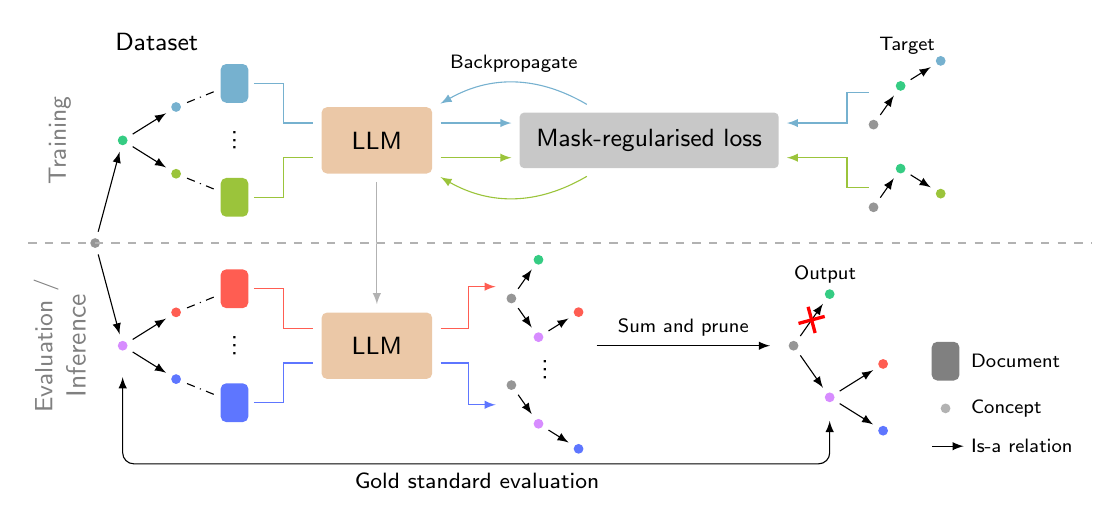
\begin{tikzpicture}
        [
            >=latex,
            doc/.style={
                    rectangle,
                    rounded corners=2pt,
                    minimum width=10pt,
                    minimum height=14pt,
                    outer sep=2pt,
                },
            llm/.style={
                    rectangle,
                    rounded corners=2pt,
                    fill={black!20},
                    minimum width=40pt,
                    minimum height=24pt,
                    outer sep=3pt,
                },
            concept/.style={
                    circle,
                    fill={black!30},
                    inner sep=1.25pt,
                    outer sep=2.5pt,
                },
            every node/.append style={font=\sffamily},
            pics/.cd,
            % Marque croix en diagonale
            Cross/.style args={#1 and #2}{%
                    code = {%
                            \draw[#2,rotate=45,scale=1.4,very thick]
                            (0,#1 pt) -- (0,-#1 pt) ;
                            \draw[#2,rotate=-45,scale=1.4,very thick]
                            (0,#1 pt) -- (0,-#1 pt) ;
                        }
                },
            Cross/.default={2.5 and gray!25!black},
        ]
        \newcommand{\nodeDist}{0.8}
        \newcommand{\nodeDistShort}{0.6}
        \newcommand{\angleA}{15}
        \newcommand{\angleB}{58}
        \definecolor{c0}{RGB}{150, 150, 150}
        \definecolor{c1}{RGB}{255, 93, 82}
        \definecolor{c2}{RGB}{94, 118, 255}
        \definecolor{c3}{RGB}{118, 177, 207}
        \definecolor{c4}{RGB}{215, 140, 255}
        \definecolor{c5}{RGB}{155, 196, 59}
        \definecolor{c6}{RGB}{53, 204, 131}
        \definecolor{llmcolor}{RGB}{235, 200, 167}
        \definecolor{losscolor}{RGB}{200, 200, 200}

        % PART A: Ontology
        \node[concept,color=c0] (root) {};
        \node[concept,color=c4] (l1) at ($(root) + ({-90+\angleA}:{\nodeDist+0.55})$) {};
        \node[concept,color=c6] (l2) at ($(root) + ({90-\angleA}:{\nodeDist+0.55})$) {};
        \node[concept,color=c1] (l11) at ($(l1) + ({90-\angleB}:{\nodeDist})$) {};
        \node[concept,color=c2] (l12) at ($(l1) + ({-90+\angleB}:{\nodeDist})$) {};
        \node[concept,color=c3] (l21) at ($(l2) + ({90-\angleB}:{\nodeDist})$) {};
        \node[concept,color=c5] (l22) at ($(l2) + ({-90+\angleB}:{\nodeDist})$) {};
        % \node[concept] (l1) at ($(root) + ({180+\angleA}:{\nodeDist})$) {};
        % \node[concept] (l2) at ($(root) + ({-\angleA}:{\nodeDist})$) {};
        % \node[concept] (l11) at ($(l1) + ({180+\angleB}:{\nodeDist})$) {};
        % \node[concept] (l12) at ($(l1) + ({-\angleB}:{\nodeDist})$) {};
        % \node[concept] (l21) at ($(l2) + ({180+\angleB}:{\nodeDist})$) {};
        % \node[concept] (l22) at ($(l2) + ({-\angleB}:{\nodeDist})$) {};
        \draw[->] (root) -- (l1);
        \draw[->] (root) -- (l2);
        \draw[->] (l1) -- (l11);
        \draw[->] (l1) -- (l12);
        \draw[->] (l2) -- (l21);
        \draw[->] (l2) -- (l22);

        \node[anchor=west,inner sep=0,align=left] (caption) at ($(root.west) + (0.4, 2.55)$) {\small Dataset};

        \newcommand{\docSpace}{0.66}
        \node[doc,fill=c1] (doc1) at ($(l11) + ({90-\angleB-10}:{\nodeDist})$) {};
        \node[doc,fill=c2] (doc2) at ($(l12) + ({-90+\angleB+10}:{\nodeDist})$) {};
        \node[doc,fill=c3] (doc3) at ($(l21) + ({90-\angleB-10}:{\nodeDist})$) {};
        % \node[doc,fill=c4] (doc4) at ($(l11) + (\docSpace, -1.5)$) {};
        \node[doc,fill=c5] (doc7) at ($(l22) + ({-90+\angleB+10}:{\nodeDist})$) {};
        \node[doc,rotate=90] (doc5) at ($(doc1)!0.5!(doc2)$) {...};
        \node[doc,rotate=90] (doc6) at ($(doc3)!0.5!(doc7)$) {...};
        \draw[dashdotted] (l11) to (doc1);
        \draw[dashdotted] (l12) to (doc2);
        \draw[dashdotted] (l21) to (doc3);
        \draw[dashdotted] (l22) to (doc7);
        % \draw[dashdotted,bend right] (l1) to (doc4);

        % line to separate the ontology into train and test
        % \draw[dashed] ($(root) + (0, 0.4)$) -- ($(root) + (0, -2.6)$);
        % \node at ($(root) + (1.1, -0.1)$) {Train};
        % \node at ($(root) + (-1.1, -0.1)$) {Test};

        % \draw[dashed] ($(root) + (-0.4, 0)$) -- ($(root) + (2.0, 0)$);
        % \node[anchor=west,inner sep=0] at ($(root.west) + (0, 1.1)$) {\small Train};
        % \node[anchor=west,inner sep=0] at ($(root.west) + (0, -1.5)$) {\small Test};

        % PART B: Training
        \newcommand{\vertSpace}{0.22}
        \newcommand{\trainSpace}{0.7}
        % \node[doc,fill=c3] (input) at ($(doc3) + (1.0, 0)$) {};
        % \node[doc,fill=c5] (inputp) at ($(doc7) + (1.0, 0)$) {};

        \node[llm,anchor=west,fill=llmcolor] (llm) at ($(doc3)!0.5!(doc7) + (1, 0)$) {\small LLM};
        \node[anchor=west,align=center,rounded corners=1.5pt,outer sep=3pt,inner sep=6pt,fill=losscolor] (loss) at ($(llm.east) + (\trainSpace + 0.2, 0)$) {\small Mask-regularised loss};

        \begin{scope}[local bounding box=target1,shift={($(loss.east) + (1.1, 0.2)$)},outer sep=3pt]
            \node[concept,color=c0] (sgRoot) {};
            \node[concept,color=c6] (sg2) at ($(sgRoot) + ({90-\angleA-20}:{\nodeDistShort})$) {};
            \node[concept,color=c3] (sg21) at ($(sg2) + ({90-\angleB}:{\nodeDistShort})$) {};
            \draw[->] (sgRoot) -- (sg2);
            \draw[->] (sg2) -- (sg21);
        \end{scope}

        \begin{scope}[local bounding box=target2,shift={($(loss.east) + (1.1, -0.85)$)},outer sep=3pt]
            \node[concept,color=c0] (sgRoot) {};
            \node[concept,color=c6] (sg2) at ($(sgRoot) + ({90-\angleA-20}:{\nodeDistShort})$) {};
            \node[concept,color=c5] (sg22) at ($(sg2) + ({-90+\angleB}:{\nodeDistShort})$) {};
            \draw[->] (sgRoot) -- (sg2);
            \draw[->] (sg2) -- (sg22);
        \end{scope}

        \coordinate (out) at ($(llm.west) + (0, \vertSpace)$);
        \draw[color=c3] (doc3) -| ($(doc3.east)!0.5!(out)$) |- (out);
        \draw[->,color=c3] ($(llm.east) + (0, \vertSpace)$) -- ($(loss.west) + (0, \vertSpace)$);

        \coordinate (out) at ($(llm.west) + (0, -\vertSpace)$);
        \draw[color=c5] (doc7) -| ($(doc7.east)!0.5!(out)$) |- (out);
        \draw[->,color=c5] ($(llm.east) + (0, -\vertSpace)$) -- ($(loss.west) + (0, -\vertSpace)$);

        \coordinate (out) at ($(loss.east) + (0, \vertSpace)$);
        \draw[->,color=c3] (target1) -| ($(target1)!0.5!(out)$) |- (out);
        \coordinate (out) at ($(loss.east) + (0, -\vertSpace)$);
        \draw[->,color=c5] (target2) -| ($(target2)!0.5!(out)$) |- (out);
        \draw[->,bend right,color=c3] (loss) to node [midway,above,align=center,color=black] {\scriptsize Backpropagate} (llm);
        \draw[->,bend left,color=c5] (loss) to (llm);
        \node at ($(target1) + (0, 0.6)$) {\scriptsize Target};

        % PART C: Inference
        \node[llm,anchor=west,fill=llmcolor] (llm1) at ($(doc1)!0.5!(doc2) + (1.0, 0)$) {\small LLM};
        % \node[doc,fill=c1,anchor=east] (input1) at ($(llm1.west) + (-\trainSpace, 0.8)$) {};

        \begin{scope}[local bounding box=sg1,shift={($(llm1.east) + (\trainSpace + 0.2, 0.6)$)}]
            \node[concept,color=c0] (sgRoot1) {};
            \node[concept,color=c4] (sg11) at ($(sgRoot1) + ({-90+\angleA+20}:{\nodeDistShort})$) {};
            \node[concept,color=c6] (sg12) at ($(sgRoot1) + ({90-\angleA-20}:{\nodeDistShort})$) {};
            \node[concept,color=c1] (sg112) at ($(sg11) + ({90-\angleB}:{\nodeDistShort})$) {};
            \draw[->] (sgRoot1) -- (sg12);
            \draw[->] (sgRoot1) -- (sg11);
            \draw[->] (sg11) -- (sg112);
        \end{scope}

        \begin{scope}[local bounding box=sg2,shift={($(llm1.east) + (\trainSpace + 0.2, -0.5)$)}]
            \node[concept,color=c0] (sgRoot2) {};
            \node[concept,color=c4] (sg21) at ($(sgRoot2) + ({-90+\angleA+20}:{\nodeDistShort})$) {};
            \node[concept,color=c2] (sg211) at ($(sg21) + ({-90+\angleB}:{\nodeDistShort})$) {};
            \draw[->] (sgRoot2) -- (sg21);
            \draw[->] (sg21) -- (sg211);
        \end{scope}


        % \node (dots) at ($(input1)!0.5!(input2)$) {...};
        % \node (dots2) at ($(dots) + (4.0, 0)$) {...};
        \node[rotate=90] at ($(sg1)!0.5!(sg2) + (0, -0.15)$) {...};
        \draw[color=c1] (doc1) -| ($(doc1.east)!0.5!(llm1.west)$) |- ($(llm1.west) + (0, \vertSpace)$);
        \coordinate (out1) at ($(llm1.east) + (\trainSpace, 0.75)$);
        \draw[->,color=c1] ($(llm1.east) + (0, \vertSpace)$) -| ($(llm1.east)!0.5!(out1)$) |- (out1);
        \draw[color=c2] (doc2) -| ($(doc2.east)!0.5!(llm1.west)$) |- ($(llm1.west) + (0, -\vertSpace)$);
        \coordinate (out2) at ($(llm1.east) + (\trainSpace, -0.75)$);
        \draw[->,color=c2] ($(llm1.east) + (0, -\vertSpace)$) -| ($(llm1.east)!0.5!(out2)$) |- (out2);


        % \node[doc,fill=c1] (input1) at ($(input) + (0, -2.0)$) {};
        % \node[llm] (llm1) at ($(input1) + (\trainSpace, 0)$) {LLM};
        % \node[concept] (sgRoot1) at ($(llm1) + (\trainSpace + 0.8, 0.6)$) {};
        % \node[concept] (sg11) at ($(sgRoot1) + ({180+\angleA}:{\nodeDist})$) {};
        % \node[concept] (sg12) at ($(sgRoot1) + ({-\angleA}:{\nodeDist})$) {};
        % \node[concept] (sg111) at ($(sg11) + ({180+\angleB}:{\nodeDist})$) {};
        % \draw[->] (input1) -- (llm1);
        % \draw[->] (llm1) -- ($(llm1) + (\trainSpace-0.25, 0)$);

        % \node[doc,fill=c2] (input2) at ($(input1) + (0, -1.7)$) {};
        % \node[llm] (llm2) at ($(input2) + (\trainSpace, 0)$) {LLM};
        % \node[concept] (sgRoot2) at ($(llm2) + (\trainSpace + 0.8, 0.6)$) {};
        % \node[concept] (sg21) at ($(sgRoot2) + ({180+\angleA}:{\nodeDist})$) {};
        % \node[concept] (sg212) at ($(sg21) + ({-\angleB}:{\nodeDist})$) {};
        % \draw[->] (input2) -- (llm2);
        % \draw[->] (llm2) -- ($(llm2) + (\trainSpace-0.25, 0)$);

        \node[concept,color=c0] (testOutRoot) at ($(doc1)!0.5!(doc2) + (7.1, 0.0)$) {};
        \node[concept,color=c4] (testOut1) at ($(testOutRoot) + ({-90+\angleA+20}:{\nodeDist})$) {};
        \node[concept,color=c2] (testOut11) at ($(testOut1) + ({-90+\angleB}:{\nodeDist})$) {};
        \node[concept,color=c1] (testOut12) at ($(testOut1) + ({90-\angleB}:{\nodeDist})$) {};
        \node[concept,color=c6] (testOut2) at ($(testOutRoot) + ({90-\angleA-20}:{\nodeDist})$) {};
        \node at ($(testOutRoot) + (0.4, 0.9)$) {\scriptsize Output};
        \draw[->] (testOutRoot) -- (testOut1);
        \draw[->] (testOut1) -- (testOut11);
        \draw[->] (testOut1) -- (testOut12);
        \draw[->] (testOutRoot) -- pic[midway,-,rotate=60] {Cross={3.5 and red}} (testOut2);
        \draw[->] ($(doc1)!0.5!(doc2) + (4.6, 0)$) -- node [midway,above,align=center] {\scriptsize Sum and prune} ($(doc1)!0.5!(doc2) + (6.8, 0)$);

        % PART D: Evaluation
        \coordinate (start) at ($(l1) + (0, -0.4)$);
        \coordinate (inter) at ($(start) + (4.5, -1.1)$);
        \coordinate (end) at ($(testOut1) + (0, -0.3)$);
        \draw[<->,rounded corners] (start) |- (inter) -| (end);
        \node[below] at (inter) {\footnotesize Gold standard evaluation};

        % Draw a separation line between Part B and Part C
        \draw[color={black!30},dashed] ($(root) + (-0.85, 0)$) -- ($(root) + (12.65, 0)$);
        % Caption Part B
        \node[color={black!50},inner sep=0,rotate=90] at ($(l2) + (-0.8, 0)$) {\small Training};
        % Caption Part C
        \node[color={black!50},inner sep=0,rotate=90,align=center] at ($(l1) + (-0.8,0)$) {\small Evaluation /\\Inference};
        % Arrow connection llm train to llm inference.
        \draw[->,color={black!30}] (llm) |- ($(llm)!0.5!(llm1)$) -| (llm1);
        % Legend
        \node[doc,fill={black!50}] (docLegend) at ($(root) + (10.8, -1.5)$) {};
        \node[anchor=west] (docDesc) at ($(docLegend) + (0.2, 0)$) {\scriptsize Document};
        \node[concept] (conceptLegend) at ($(docLegend) + (0, -0.6)$) {};
        \node[anchor=west] (conceptDesc) at ($(conceptLegend) + (0.2, 0)$) {\scriptsize Concept};
        \node (arrow1) at ($(docLegend.west) + (-0.05, -1.08)$) {};
        \node (arrow2) at ($(arrow1) + (0.65, 0)$) {};
        \draw[->] (arrow1) -- (arrow2);
        \node[anchor=west] (arrowDesc) at ($(conceptDesc.west) + (0, -0.47)$) {\scriptsize Is-a relation};
    \end{tikzpicture}
    \caption{\name: Using annotations of documents with their relevant concepts, we train an LLM to model relevant subgraphs of the target ontology with a custom regulariser. During inference, the generated subgraphs for each document are summed and pruned to give the final output ontology. For evaluation, we measure the similarity between the generated ontology and the ground truth.}
    \label{fig:overview}
\end{figure}

% \begin{figure}
%     \centering
%     \includegraphics[width=0.8\linewidth]{media/Finetune masked_test_output.pdf}
%     \caption{\todo{Really hard to embed the whole graph while still readable... Perhaps just show a subgraph and include the full graph in the appendix.}}
%     \label{fig:enter-label}
% \end{figure}

An ontology is a formal and structural way of representing domain-specific concepts and their relations~\cite{gruber1995toward}.
They can be simple (e.g., Wikipedia categories) consisting of \emph{concepts} and only a small number of types of \emph{taxonomic relations} (e.g., \emph{is-a} relationships), or they can be complex (e.g., Schema.org) consisting of axioms or many types of relations. For example, a simple ontology for programming languages might contain two concepts ``Dynamically-typed language'' and ``Python'', and one relation ``Dynamically-typed language $\to$ Python'', representing the knowledge that Python is a dynamically-typed language. A more complex ontology might contain axioms too, for example, ``all programming languages are either dynamically or statically typed''.
In this paper, we focus on ontologies with only concepts and taxonomic relations. Compared to typical deep learning models, which represent knowledge implicitly in its weights, ontologies capture knowledge in a structured and explicit manner, making them reliable, easy to edit and human-interpretable. Such benefits of ontologies have led to their wide adoption in practice. For example, Wikipedia categories have been used for entity ranking~\cite{vercoustre2008using} and information retrieval~\cite{sorg2012exploiting}, or Schema.org~\cite{Schema.org_2011} is a core component of the Semantic Web~\cite{antoniou2004semantic} initiative.

While ontologies are useful, building ontologies often requires substantial manual effort. Ontology learning (OL) is the study of automating the construction of high-quality ontologies at scale. For a simple ontology, this amounts to discovering the concepts and taxonomic relations, usually based on a source corpus. In this paper we aim to develop domain-independent methods for OL that are scalable and produce better ontologies.

Traditionally, OL is viewed as a composition of subtasks~\cite{asim2018survey}, such as concept discovery and relation extraction. In particular, prior works have demonstrated that state-of-the-art large language models (LLMs) can solve such subtasks effectively~\cite{babaei2023llms4ol}. While studying subtasks permits fine-grained analysis and evaluation, it does not directly indicate the subsequent impact on the quality of the final ontology. Moreover, there is potential room for improvement by combining several subtasks into one, such as by modelling concepts and relations in conjunction. In this paper, we instead develop and evaluate methods that construct ontologies in an end-to-end fashion to answer the following research questions:
\begin{enumerate}[itemsep=0pt,leftmargin=*]
    \item How can we leverage LLMs' knowledge base to build ontologies from scratch?
    \item Does our method scale efficiently to practical problem sizes?
    \item How well does our method generalise to new domains?
\end{enumerate}

We introduce \name, an end-to-end method for using LLMs to construct ontologies at scale. Rather than focusing on individual relations between concepts, we finetune an LLM to model entire sub-components of the target ontology. The output ontology is generated by taking the sum of generated sub-components and applying simple post-processing. An overview of the pipeline is shown in \cref{fig:overview}. To train \name, we collect the categorisation metadata for a subset of Wikipedia articles. We attempt to adapt an LLM to model the relevant categorisation subgraph for a particular Wikipedia article, but discover that direct finetuning leads to poor generalisation due to overfitting to high-level, frequently occurring concepts. Instead, we propose a custom regulariser that reweights each concept based on its frequency of occurrence, which substantially improves generalisation.

We evaluate \name by measuring the similarity of the generated ontology with the ground truth. Current approaches for comparing ontologies rely on mapping components of the two ontologies onto each other, most commonly by literal text matching \cite{maedche2002measuring,Treeratpituk2013GraphbasedAT}. This is unreliable when the two ontologies are not already sufficiently similar. Instead, we propose a suite of evaluation metrics suitable for comparing arbitrary labelled graphs. These metrics compare edges and subgraphs of the two ontologies using pretrained text embedders to test for semantic and structural similarity. Both our quantitative and qualitative results reveal that an LLM can already outperform existing extraction-based methods out of the box, and the performance is further improved by finetuning with our custom regulariser. We additionally demonstrate that \name can be adapted to build the arXiv ontology using only a small number of training examples, suggesting that our model can be applied to new domains in a data-efficient way. In summary, our contributions are:
\begin{enumerate}[itemsep=0pt,leftmargin=*]
    \item We constructed two datasets based on Wikipedia and arXiv, which can serve as standard datasets for future work studying end-to-end OL.
    \item We created \name, a method that utilises LLMs to build ontologies from scratch. \name produces high-quality ontologies and serves as a strong baseline for end-to-end OL.
    \item We developed new evaluation metrics for assessing the quality of the generated ontologies.
\end{enumerate}

\section{Background}

% \subsection{Ontology learning}
% Key points:
% \begin{enumerate}
%     \item Explain what an ontology is. State that we only focus on constructing a simplistic ontology (with just classes and taxonomic relation). 
%     \item Give a brief overview of non-LM-based approaches. In particular Hearst patterns \cite{hearst1998automated}.
%     \item Given an overview of LM-based methods. State their shortcomings. First efforts by \citet{petrucci2016ontology,petrucci2018expressive} viewing OL as a translation task from natural language to Description Logic formulae. It is only tested on synthetic datasets and a small number of manually curated examples due to the lack of such a natural language-description language pairing dataset. \citet{babaei2023llms4ol} benchmarked LLMs for several subtasks of OL such as link prediction. There exists proof-of-concept end-to-end methods using LLMs by recursive prompting \cite{funk2023towards} or generating entire ontology directly in one generation prompt \cite{trajanoska2023enhancing}, both of which only considered graphs up to $\approx$1000 nodes and relied on manual evaluation. \todo{Include clustering-based approaches?} \todo{Some of these should go into ``related works''.}
% \end{enumerate}
%
% Key points:
% \begin{enumerate}
%     \item Introduce any mathematical notations here, e.g., $G=(V,E)$ for a graph.
%     \item Assume we have a ground truth ontology represented as a directed graph, where nodes represent classes and edges represent taxonomic relations. Each node has a label in natural language and is optionally associated with one or more documents, which in our case is represented by a title and some main body text. The goal is to recover the graph given the set of documents. 
% \end{enumerate}
%
% [What is an ontology and how is it represented?]
An ontology is a structured way of representing concepts and relations of a shared conceptualisation, that is, domain knowledge~\cite{gruber1995toward,gruber1993translation}. In this paper, we focus on ontologies that only consist of concepts and taxonomic relations which represent \emph{is-a} or \emph{is-subclass-of} relationships between concepts. In some cases, the \emph{is-part-of} relation is also considered a taxonomic relation. We treat such an ontology as a rooted labelled directed graph where nodes represent concepts, edges represent taxonomic relations and the root node is the special concept of all concepts. A strict ontology asserts that the taxonomic relation is asymmetric and thus the graph must be acyclic, though in practice some ontologies, such as the Wikipedia ontology studied in this paper, may contain cycles. We therefore do not assume that an ontology graph is necessarily acyclic. Examples of ontologies include WordNet~\cite{miller1995wordnet} with 117,659 concepts and 89,089 taxonomic relations, and the Gene Ontology~\cite{ashburner2000gene} with 42,255 concepts and 66,810 taxonomic relations.

% [What is the precise task we study in this paper?]
Ontology learning is the automatic extraction of ontological elements~\cite{hazman2011survey}. The most studied source of input is unstructured text, though there are also works on semi-structured data like HTML~\cite{karoui2004ontology}. In this paper, the input is a set of documents, each consisting of some unstructured text. We additionally assume each document is associated with one or more concepts in the ground truth ontology, which we utilise for training. The goal is to reconstruct the ground truth ontology given the set of documents.%\looseness-1 

% [Traditional approaches to OL.]
Prior works view OL as a composition of subtasks, and study each subtask in isolation~\cite{buitelaar2005ontology,asim2018survey}. A typical pipeline for building a simple ontology is to first perform concept discovery (identify the nodes), and then relation extraction (identify the edges)~\cite{cimiano2005text2onto,kaushik2018automatic}. A notable approach for relation extraction is Hearst patterns~\cite{hearst1998automated}. Hearst patterns are hand-crafted lexico-syntactic patterns that exploit natural language structure to discover taxonomic relations. For example, the pattern ``[noun phrase] such as [noun phrase]'' matches phrases like ``dogs such as chihuahuas'', and thus can be processed by regular expressions to identify the relation ``dog $\to$ chihuahua''. Hearst patterns suffer from low recall, as the relations must occur in exact configurations to be identified by the rules. \citet{roller2018hearst} suggests smoothing techniques to alleviate this issue though at the cost of lower precision.
% Another approach for relation extraction utilises word co-occurrence statistics to predict taxonomic relations \cite{cimiano2005learning}.

% [LLM approaches to OL]
Recently, language models have been used for OL. REBEL~\cite{cabot2021rebel} treats relation discovery as a translation task, and finetunes encoder-decoder LLMs to extract both taxonomic and non-taxonomic relations. \citet{babaei2023llms4ol} benchmarked a wide family of LLMs for concept and relation discovery, and showed promising results. There are also proof-of-concept works for building ontologies end-to-end with LLMs. \citet{funk2023towards} proposes to build an ontology by recursively prompting  LLMs, while \citet{trajanoska2023enhancing} generate the entire ontology in one completion. However, both studies are limited in the scale of the task and evaluation: they only considered ontologies of up to 1000 concepts and relied on manual qualitative evaluation. We bridge this gap by proposing a method that can scale to practical problem sizes and new metrics for systematic qualitative evaluation.

% [Prior approaches to evaluating OL.]
The evaluation of ontologies is an open research area. The main approaches are gold standard evaluation~\cite{Zavitsanos2011GoldSE}, which matches elements of the generated ontology with a predefined target ontology; task-based evaluation~\cite{porzel2004task}, which measures the usefulness of the ontology on a specific application; and human evaluation \cite{raad2015survey,brank2005survey}. In this paper, we evaluate by the gold standard metric as it is the most straightforward approach when ground-truth ontology exists. Prior works have considered matching concepts~\cite{maedche2002measuring} and direct or indirect relations~\cite{Kashyap2005TaxaMinerAE, Treeratpituk2013GraphbasedAT} by literal text comparison. Others have also considered edit-distance~\cite{Ehrig2005SimilarityFO} or bag-of-words distributional similarity for text comparison~\cite{Zavitsanos2011GoldSE}.  These techniques for measuring semantic similarity may be considered unreliable and have been superseded by current methods~\cite{conneau2017supervised}. We instead rely on more modern techniques like pretrained text embedders \cite{devlin2018bert} and graph convolutions \cite{kipf2016semi} to match substructures between the two ontologies.

% \subsection{Knowledge graph construction with LLMs \todo{Move to ``related works''?}}
% Key points:
% \begin{enumerate}
%     \item There is a lot of overlap between knowledge graph construction and OL but state the differences: KG focuses on the structured representation of facts from the source corpus, hence typically involves more types of relations and less concerned about graph structure.
%     \item Overview of methods for KG construction. Most common task is KG completion: Given a head node and a relation, predict the tail node. \citet{petroni2019language} first to use LLMs for this task by prompting. Recent work by \citet{yao2023exploring} finetunes LLMs for link prediction and relation prediction. \citet{wang2020language} inspects the attention patterns of LLMs to extract the relation token(s) between two entities in the source text.
% \end{enumerate}

\section{\name}

We now introduce \name, our novel, simple and scalable method for end-to-end OL with LLMs. On a high level, \name uses an LLM to model concept subgraphs of the target ontology by utilising a linearisation scheme to transform subgraphs into string sequences. In contrast to learning individual edges, modelling subgraphs allows the model to learn higher-order structures, such as the interactions between three or more nodes. To create the training dataset, \name relies on the annotations of documents to concepts to generate document-subgraph pairings. Such subgraphs are much smaller than the complete graph, so they can be learned by the model more easily. The generated subgraphs for each document are summed into a weighted graph, and simple post-processing is applied to obtain the final predicted ontology.

% Highlight the core components and insights for \name.
% \begin{enumerate}
%     \item The idea to model subgraphs instead of edges. Motivation: More efficient inference, captures the global structure of an ontology (the hierarchical structure is "baked in").
%     \item Components: 1. Document $\to$ subgraph. 2. Aggregrate subgraphs induced by each document into a weighted global graph. 3. Apply post-processing and pruning.
%     \item Argue that this setup is appealing for scaling: Inference can be parallelised across the source documents, so inference duration is inversely proportional to the amount of hardware available. 
% \end{enumerate}

\subsection{Subgraph modelling}  \label{sec:method:subgraph}

\begin{figure}[t]
    \centering
    \begin{subfigure}[c]{0.34\textwidth}
        \centering
        \fbox{
        \includegraphics[width=\linewidth,trim={1.5cm 1.5cm 1.5cm 1.5cm},clip]{media/Hybridity.pdf}
        }
    \end{subfigure}%
    \hfill
    \begin{adjustbox}{varwidth=\linewidth,fbox}
    \begin{subfigure}[c]{0.55\textwidth}
        \centering
        \lstdefinestyle{prompt}{
          basicstyle=\small\ttfamily\color{black},
          moredelim=**[is][\color{gray}]{@}{@},
        }
        \begin{lstlisting}[gobble=8,style=prompt]
        @<s>[INST] Title: Hybridity
        Hybridity, in its most basic sense ... [/INST]@
        Main topic classifications -> @Human behavior@ -> @Human activities@ -> Culture -> Sociology of culture
        Main topic classifications -> @Humanities@ -> Politics -> @Politics by issue@ -> @Politics and race@
        Main topic classifications -> @Politics@ -> @Politics by issue@ -> Politics and race
        Main topic classifications -> @Culture@ -> Sociology of culture</s>
        \end{lstlisting}
    \end{subfigure}
    \end{adjustbox}
    \caption{Example subgraph induced by the Wikipedia page ``Hybridity'' (left), where $N = 4$ and $C = \{\text{Politics and race}, \text{Sociology of culture}\}$.
    The corresponding training text sequence (right), where text coloured in grey is ignored as training targets but is still present as context for later tokens.}
    \label{fig:prompt-template}
\end{figure}

Here, we describe the method for creating document-subgraph pairings. Given a document and its associated set of concepts $C$, we define the \emph{relevant paths} as the set of paths of at most length $N$ from the root to any of the concepts in $C$. The \emph{relevant subgraph} is the set of nodes (concepts) and edges (taxonomic relations) that occur at least once in the relevant paths. An example is shown in \cref{fig:prompt-example} (left). The choice of $N$ is task-specific and we describe our method for choosing $N$ in \cref{sec:implementation}.

To employ LLMs to model the subgraphs, we must linearise the graph into a string sequence. Existing methods for autoregressive graph generation employ BFS \cite{you2018graphrnn} or DFS \cite{goyal2020graphgen} ordering starting at an arbitrary node. We instead choose to linearise the subgraph as a list of relevant paths that produced the subgraph in the first place. We do so over BFS/DFS ordering for three reasons: 1)~the subgraph is defined from the relevant paths, which makes them the most natural representation; 2)~we hypothesise that the hierarchy of concepts in each path is a desirable inductive bias for the hierarchical nature of an ontology; and 3)~the path-based representation is much easier to describe in natural language instructions so that our LLM prompting-based baselines may produce reasonable results without finetuning. The linearisation template can be found in \cref{fig:linearisation-template} in Appendix~\ref{appendix:training-details}.

% Key points:
% \begin{enumerate}
%     \item Explain how to construct document-subgraph pairing from the training dataset. E.g., the path length cutoff is selected as the smallest number that still covers almost all of the edges.
%     \item Linearisation of subgraph to a sequence. Why choose the method of ``subgraph as a set of paths''? Ans: More natural language-like, easier for zero/few-shot to comprehend so we have stronger baselines.
%     \item \fig{Example output format.}
% \end{enumerate}

\subsection{Post-processing}  \label{sec:method:post-processing}

The final output graph is obtained by summing all generated subgraphs for each document and pruning low-weighted components. Given the generated subgraphs $G_1 = (V_1, E_1), \dots, G_n = (V_n, E_n)$, the raw output graph is defined as $G_\text{raw} = (V_\text{raw}, E_\text{raw})$, where $V_\text{raw} = \cup_{i=1}^n V_n$ and $E_\text{raw} = \cup_{i=1}^n E_n$. Each edge $(u, v) \in E_\text{raw}$ is additionally weighted by the number of times it occurs in the collection of subgraphs: $w(u, v) = \sum_{i=1}^n \mathbbm{1}[(u,v) \in E_n]$. A few simple post-processing steps are then applied to $G_\text{raw}$ in order to prune it:
\begin{enumerate}[itemsep=1pt,leftmargin=*]
    \item Self-loop pruning: All edges $(u, u) \in E_\text{raw}$ are removed.
    \item Inverse-edge pruning: For $(u, v) \in E_\text{raw}$, if $(v, u) \in E_\text{raw}$ and $w(v, u) > w(u, v)$, remove $(u, v)$. That is, bidirectional edges are turned into unidirectional ones.
    \item Absolute thresholding: Edges in $E_\text{raw}$ with weight below the $\alpha$-th quantile are removed, where $0 \leq \alpha \leq 1$ is a hyperparameter. This removes edges that are globally less important.
    \item Relative thresholding: For each vertex $u \in V_\text{raw}$, let $e_1, \dots, e_k$ be the outgoing edges from $u$ sorted by weight in ascending order. Let the cumulative weight be $C(e_i) = \sum_{j=1}^i w(e_j) / \sum_{j=1}^k w(e_j)$. The edges $\{e_i\ |\ C(e_i) \leq \beta\}$ are pruned, where $0 \leq \beta \leq 1$ is a hyperparameter. This is similar to top-$p$ sampling \cite{holtzman2019curious} which we use to remove edges that are less important than their neighbours.
    \item Clean up: After pruning all edges, nodes with no incoming or outgoing edges are removed.
\end{enumerate}
%In our implementation, 
We choose the hyperparameters $\alpha$ and $\beta$ by tuning on the validation set (\cref{sec:implementation}).

% Key points:
% \begin{enumerate}
%     \item Aggregate inference outputs into a weighted directed graph.
%     \item Following \cite{roller2018hearst}, we prune self loops and edge $u \to v$ if $v \to u$ is also in the graph with a higher weight.
%     \item Apply two thresholding values to prune the graph further. The first threshold $\alpha$ where the lowest-weighted $100 \alpha\%$ of edges are pruned. The second threshold $\beta$ is a relative threshold where \emph{for each node}, the lowest-weighted outgoing edges that are in the bottom $100\beta\%$ cumulative probability mass are removed. \todo{Perhaps easier to describe in equations.}
%     \item The hyperparameters $\alpha$ and $\beta$ are tuned on the evaluation set.
% \end{enumerate}

\section{Evaluating end-to-end OL}

%Since our problem setup is uncommon in existing literature, we also develop new evaluation methods. 
Ontology evaluation is a hard problem as there are no quantitative definitions of what constitutes a ``good ontology'', and metrics generally only capture one aspect (e.g., structure but not semantics) of an ontology. We approach evaluation by treating the ground truth as a proxy for a good ontology, and comparing the generated ontologies against the ground truth. Here, we describe how the ground truth is obtained, and introduce new evaluation metrics that are used for measuring ontology similarity.

% Key points:
% \begin{enumerate}
%     \item Explain the goals of evaluation---what do we care about? Ans: Semantics and structure.
%     \item Suggest why end-to-end evaluation is hard: Large graph. Generally, a ``good ontology'' is ill-defined. Difficult to find one metric that describes all. Always trade-offs. No standard evaluation metric. 
%     \item How do we overcome this? 1. Use a ground truth ontology as a proxy for ``good ontology'' and measure how similar the generated ontology is to the ground truth. 2. Propose a series of evaluation metrics to capture various aspects of the generated output.
% \end{enumerate}

\subsection{Dataset}  \label{sec:dataset}



We collect the datasets for the two ontologies considered in this paper: Wikipedia categories and the arXiv taxonomy. We use Wikipedia for learning and in-domain evaluation, and arXiv for out-of-domain evaluation. To build the Wikipedia dataset, we perform a BFS traversal from its root category ``Main topic classifications'' up to depth 3. For every category encountered, we retrieve the titles and summaries (the text before the first section) of up to 5000 pages that belong in that category. The source data is obtained from the Wikipedia API.\footnote{\url{https://en.wikipedia.org/w/api.php}}
The arXiv taxonomy is available from its home page, and the source corpus is constructed from the title and abstract of all the papers uploaded to arXiv in the years 2020--2022 with more than or equal to 10 citations.\footnote{Citation counts obtained from \url{https://api.semanticscholar.org/}.} In total, the Wikipedia dataset has 13886 concepts, 28375 taxonomic relations and 362067 documents, while the arXiv dataset has 161 concepts, 166 taxonomic relations and 126001 documents.

\begin{figure}
    \centering
    \begin{subfigure}[t]{0.3\linewidth}
        \centering
        \includegraphics[width=\linewidth,trim={0.4cm 0.65cm 0.5cm 0.9cm},clip]{media/Wikipedia_train_eval_test_split.pdf}
        \caption{Wikipedia}
    \end{subfigure}%
    \qquad\qquad
    \begin{subfigure}[t]{0.25\linewidth}
        \centering
        \includegraphics[width=\linewidth,trim={1cm 1cm 1cm 1.2cm},clip]{media/arXiv_train_eval_test_split.pdf}
        \caption{arXiv}
    \end{subfigure}
    \caption{Intersection of concepts among the train, validation and test splits of the datasets.}
    \label{fig:dataset-overlap}
\end{figure}

Generating the train and test splits from the datasets is a non-trivial problem. Each training example consists of a document and its relevant subgraph (\cref{sec:method:subgraph}). The naive approach of randomly selecting a subset of document-subgraph pairs for the training likely leads to data leakage as there might be a significant overlap between subgraphs in the training set and the test set. Instead, we first split the full ontology into train and test graphs, and then generate the training document-subgraph pairs. This ensures that there are sufficiently many unseen concepts (and thus relations) in the test split, as shown in \cref{fig:dataset-overlap}. Our method is as follows:
\begin{enumerate}[itemsep=0pt,leftmargin=*]
    \item Let $V^\text{top}$ be the set of top-level nodes, that is, children of the root node. Randomly partition $V^\text{top}$ into train $V^\text{top}_{\text{train}}$, validation $V^\text{top}_{\text{val}}$, and test $V^\text{top}_{\text{test}}$ splits in 7:3:10 ratio.
    \item Let $d$ be the depth on the full graph, that is, the distance of the furthest node from the root. The nodes of the train graph are taken as the union of all the nodes that are within distance $d - 1$ from any node in $V^\text{top}_\text{train}$, plus $V_\text{train}^\text{top}$ and the root. The edges are all the edges in the full graph that have both endpoints in the train graph. Similar applies for $V^\text{top}_\text{val}$ and $V^\text{top}_\text{test}$.
\end{enumerate}

% Key points:
% \begin{enumerate}
%     \item Describe the data collection procedure.
%     \item Report the dataset statistics, e.g., number of nodes/edges/documents. Wikipedia: 13886 / 28375 / 362067. arXiv: 161 / 166 / 126001.
%     \item Highlight the thought process behind the creation of the train-eval-test split (Balance between the diversity of the training set and having unseen nodes/edges in the eval/test split).
%     \item \fig{Venn diagram to show the overlap between the train/eval/test splits. \cref{fig:dataset-overlap}}
% \end{enumerate}

\subsection{Metrics}

Many existing methods for comparing ontologies rely on syntactic measures like string edit distance~\cite{Ehrig2005SimilarityFO} as a proxy for semantic similarity, or require every concept to be tagged with descriptions or documents for distributional semantics comparison~\cite{Zavitsanos2011GoldSE}. To obtain more robust and general evaluation results, we introduce a suite of similarity metrics that use modern methods like text embeddings~\cite{reimers-2019-sentence-bert}. Multiple metrics are used as they trade off between interpretability and comprehensiveness, and we aim to make them complementary by capturing different aspects of an ontology. We denote the ground truth ontology graph as $G = (V, E)$ and the generated graph as $G' = (V', E')$.

\textbf{Literal~F1 }
While literal text matching is unreliable, it is also the simplest and the most interpretable. We treat this metric as a reference metric for sanity check. The Literal~F1 metric~\cite{Kashyap2005TaxaMinerAE} is given by the harmonic mean of the precision and recall of the edges:
\[
    \text{Literal precision} = \frac{|E \cap E'|}{|E'|} \qquad
    \text{Literal recall} = \frac{|E \cap E'|}{|E|}
\]

\textbf{Fuzzy~F1 }
The Literal~F1 metric puts a strong emphasis on using the correct wording, while in practice, we are interested in evaluating the semantics of an ontology. For example, using a synonymous phrase for a concept should not be penalised. We utilise embeddings from a pretrained sentence transformer \cite{reimers-2019-sentence-bert} and use the cosine similarity of the embeddings to measure semantic similarity. Specifically, let $\nodesim(u, u') \in V \times V' \to [-1, 1]$ be the cosine similarity between the sentence embeddings for $u$ and $u'$. The Fuzzy~F1 score is obtained from the fuzzy precision and recall, defined as:
\begin{equation*}
    \begin{aligned}
        \text{Fuzzy precision} & = \frac{|
            \{(u', v') \in E' \mid \exists (u, v) \in E.
            \nodesim(u, u') > t \land \nodesim(v, v') > t
            \}
        |}{|E'|}                           \\
        \text{Fuzzy recall}    & = \frac{|
            \{(u, v) \in E \mid \exists (u', v') \in E'.
            \nodesim(u, u') > t \land \nodesim(v, v') > t
            \}
        |}{|E|}                            \\
    \end{aligned}
\end{equation*}
where $t$ is the matching threshold. We use all-MiniLM-L6-v2~\cite{wang2020minilm,reimers-2019-sentence-bert} as the embedding model, and choose $t$ as the median cosine similarity between the synonyms in WordNet~\cite{miller1995wordnet}, computed as~0.436.

\textbf{Continuous~F1 }
With fuzzy comparisons, the matches between the edges of the generated and the ground truth graph are no longer one-to-one. This is problematic: consider two graphs $A\!\rightarrow\!B$ and $B\!\leftarrow\!A\!\rightarrow\!B'$, where $B$ and $B'$ match fuzzily. Such graphs will achieve a perfect Fuzzy~F1 score yet they significantly differ. Additionally, we found that the previous metrics fail to provide a useful signal for hyperparameter tuning, particularly for our baselines where the generated graphs are poor. The Continuous~F1 metric solves these issues by computing the highest-scoring edge matching between the two graphs, where the similarity score between $(u, v)$ and $(u', v')$ is given by $\min(\nodesim(u, u'), \nodesim(v, v'))$. Obtaining such matching is equivalent to solving the linear assignment problem~\cite{martello1987linear}, which can be computed by the Hungarian algorithm~\cite{kuhn1955hungarian}. The Continuous~F1 score is obtained from the continuous precision and recall, given by:
\[
    \text{Continuous precision} = \frac{s_\text{cont}}{|E'|} \qquad
    \text{Continuous recall} = \frac{s_\text{cont}}{|E|}
\]
where $s_\text{cont}$ is the score achieved by the best edge matching.

\textbf{Graph~F1 }
Instead of individual edges, this metric aims to capture the wider structure of the two graphs. Intuitively, we want to know how concepts are related to their local neighbourhood. We do so by using simple graph convolutions~\cite{wu2019simplifying} with $K=2$ to compute graph-aware node embeddings after embedding each node with the pretrained embedder. Such embeddings in $G$ are compared against those in $G'$ by cosine similarity, and the highest-scoring node matching, similar to the Continuous~F1 metric, gives the graph similarity score. The Graph~F1 score is computed from the graph precision and recall, defined as:
\[
    \text{Graph precision} = \frac{s_\text{graph}}{|V'|} \qquad
    \text{Graph recall} = \frac{s_\text{graph}}{|V|}
\]
where $s_\text{graph}$ is the score achieved by the best node matching.

\textbf{Motif distance }
Taking inspiration from classical network analysis, we use \emph{network motifs}~\cite{milo2002network,shen2002network} to evaluate the structural integrity of the generated graphs. Network motifs are reoccurring subgraphs in a larger graph, most commonly 3-vertex subgraphs. They are typically indicative of the structural characteristics of the full graph. We define the motif distance as the 1-Wasserstein distance~\cite{Kantorovich1960MathematicalMO} between the distribution of all 3-vertex subgraphs in $G$ and $G'$.

% \begin{enumerate}
%     \item Explain the rationale behind each evaluation metric.
%     \item Literal edge comparison: Simplest and most interpretable but not strongly indicative of the model's performance. For example, the solution of memorising the training split does very well.
%     \item Fuzzy edge comparison: Use embedding cosine similarity to determine a match between edges. We take the median similarity of English synonyms as the matching threshold for each endpoint. An edge matches another edge if both endpoints match.
%     \item Continuous edge matching: Solves the problem where graphs with repeated components like $B \leftarrow A \rightarrow B$ and $A \rightarrow B$ achieve a perfect score on the two metrics above. Instead, we need to compute the highest-scoring matching between the edges of the two graphs. This can be further improved by using the cosine similarity scores directly so that we can compare two graphs even when they contain no literally/fuzzily common edges.
%     \item Graph similarity matching: Previous metrics are only aware of individual edges. We want something that captures the wider structure of the graph as well. We use a simple graph convolution \cite{wu2019simplifying} to compute structure-aware node embeddings and compute the highest-scoring matching similar to continuous edge matching.
%     \item Motif distance: Taking inspiration from classical network analysis, we use \emph{network motifs} \cite{milo2002network,shen2002network} to evaluate the structural integrity of the generated graphs. Give a brief explainer of network motifs. We compute the 1-Wasserstein distance between the distribution of 3-vertex motifs identified in the generated and ground truth graph.
% \end{enumerate}

\section{Experiments}

We design our experiments to answer the following research questions:
\begin{enumerate}[itemsep=0pt,leftmargin=*]
    \item Does \name produce better ontologies than traditional methods by subtask composition?
    \item Can \name be easily adapted to a new domain?
\end{enumerate}
We approach the questions by training \name on the Wikipedia dataset, and further transfer the model to arXiv with a small number of arXiv samples. As baselines, we use two relation extraction methods, Hearst patterns~\cite{hearst1998automated,roller2018hearst} and REBEL~\cite{cabot2021rebel}. Relation extraction depends on successful concept discovery to produce high-quality ontologies. To estimate a ceiling to such baselines, \emph{we give the baselines a substantial advantage} by providing them with the ground truth concepts in the test graph. The results show that even with such an advantage, \name outperforms the baselines on many metrics, demonstrating the potential of \name for end-to-end OL (\cref{sec:results}).

\subsection{Implementation details}  \label{sec:implementation}


% \subsection{Masked loss regularisation}  \label{sec:method:masked-loss}

\begin{figure}[t]
\vspace*{-2mm}  
    \centering
    \begin{subfigure}[c]{\textwidth}
        \centering
        \includegraphics[width=\linewidth,trim={0 1cm 0 0},clip]{media/vanilla.png}
        
        \vspace*{-1mm}
        \caption{Direct finetuning}
    \end{subfigure}%
    \hfill
    \begin{subfigure}[c]{\textwidth}
        \centering
        \includegraphics[width=\linewidth,trim={0 1cm 0 0},clip]{media/masked.png}
        
        \vspace*{-1mm}  
        \caption{Finetuning with masked loss}
    \end{subfigure}%
    \caption{Per token loss on a test set example of the final model trained with and without the custom masked loss objective. Within the top-level concepts (children of the root) shown here, ``Culture'' and ``Humanities'' are in the training set while others are not. Using the masked loss objective improves generalisation on the high-level relations while maintaining performance on lower-level relations.}
    \label{fig:vanilla-vs-mask}
    \vspace*{-2mm}  
\end{figure}

%We discover that directly finetuning an LLM on the sequences defined in \cref{sec:method:subgraph} produces poor results due to overfitting. 
Analysing the per-token loss on the test split sequences of a directly finetuned model (\cref{sec:method:subgraph}) shows that the model tends to memorise high-level relations from the training set, leading to poor generalisation, as shown in \cref{fig:vanilla-vs-mask} (top).
% This occurs because high-level relations are present in many relevant subgraphs and thus repeated many times in the training set.
% This problem is not solvable by early stopping since terminating training early will result in a model that massively underfits lower-level relations.
% This issue is akin to multi-task learning \cite{caruana1997multitask} as the model trying to learn both high and low-level concepts simultaneously
% where the standard solution is to apply some loss weighting factor to rebalance training objectives \cite{sermanet2013overfeat, kendall2018multi}.
The crux of the problem is that low-level relations are substantially more diverse than high-level ones: since we present both types of relations at the same rate to the model, it tends to overfit on high-level relations while underfitting on low-level ones.
To alleviate this issue, we introduce a new training objective that randomly masks the loss contribution of frequently occurring relations. Suppose a relation $u \to v$ is present $n$ times in the training set. During training, when $u \to v$ appears in one of the relevant paths, we mask the loss contribution of the tokens for $v$ with probability $\max(1 - \nicefrac{M}{n}, 0)$, where $M$ is a constant for the average number of times a relation is present in the training set. Intuitively, this regulariser ensures that frequent relations are only seen $\approx\!M$ times as targets throughout training, hence reducing overfitting as shown in \cref{fig:vanilla-vs-mask} (bottom). Note that while $v$ is masked from the target, its tokens are still present in the input sequence as context for later tokens. A concrete training example can be found in \cref{fig:prompt-example} (right).

We finetune Mistral 7B v0.2~\cite{jiang2023mistral} with Low-Rank Adaptation~\cite{hu2021lora} on the masked loss objective. The model is trained on the Wikipedia dataset for two epochs with Adam. During inference, the outputs are generated with temperature 0.1 and nucleus sampling~\cite{holtzman2019curious} top-$p$ of 0.9. We include a finetuning baseline without the masked loss objective, denoted as Finetune. To adapt \name for arXiv, we further finetune the model on 2048 document-subgraph pairs from arXiv. We initialise new low-rank adaptors and train until the loss stops improving on the validation set. We name these models \name (transfer) and Finetune (transfer) for training with and without the masked loss objective, respectively. Full details for the Wikipedia and arXiv experiments can be found in~\cref{appendix:training-details}.

The hyperparameters for the post-processing steps are tuned by grid search on the validation set. We sweep over $\alpha \in 1 - \text{geomspace}(1 / |E_\text{raw}|, 1, 21)$ and $\beta \in \text{geomspace}(0.1, 1, 21) - 0.1$ and use the values that maximise Continuous~F1. For Wikipedia, we choose the subgraph modelling path length $N=4$ as it is the smallest $N$ such that almost all edges ($>99\%$) occur in at least one relevant subgraph. Such criterion is used since smaller $N$ results in smaller subgraphs, which we expect to be easier to model accurately. We choose $N=3$ for arXiv for the same reason.

\subsection{Baselines}

We give a brief overview of the baseline methods here. The full implementation details can be found in \cref{appendix:exp-details}. All baselines produce weighted directed graphs which we apply the same post-processing steps as \name (\cref{sec:method:post-processing}) to obtain the final predicted graph.

\textbf{Memorisation }
Simply memorising the train graph is a surprisingly strong baseline due to the overlap between train and test graphs, especially for Wikipedia. The weight of each edge is given by the number of relevant subgraphs in which it appears.

\textbf{Hearst }
We follow the improved implementation of Hearst patterns by \citet{roller2018hearst}. The authors propose spmi, a method which uses low-rank approximations to smooth the relation matrix so that two concepts can be compared even if there are no direct matches between them. We use the smoothed relation matrix to weigh the relations between the ground truth concepts. The additional hyperparameter for the rank of the smoothed matrix is tuned by grid search over the validation set.

\textbf{REBEL }
The REBEL-large model~\cite{cabot2021rebel} is an LLM trained to extract many types of relations from Wikipedia articles. We only take the ``subclass of'', ``instance of'', ``member of'' and ``part of'' relations that were extracted. Similar to Hearst, we find that it fails to find many direct relations between ground truth concepts. The same low-rank smoothing technique is applied to improve recall.

\textbf{Prompting }
We test the Zero/One/Three-shot performance of instruction-tuned LLMs on the subgraph modelling task described in \cref{sec:method:subgraph}. To obtain more comparable results, we use Mistral 7B Instruct v0.2, the instruction-tuned version of the base model of \name, as the LLM for our prompting baseline. The prompt template used is shown in \cref{fig:prompt-template} in Appendix~\ref{appendix:exp-details}.

\subsection{Results}  \label{sec:results}

%\begin{table}[t]
\caption{\todo{End with a take home message}}
\label{table:metrics}
\centering
\begin{tabularx}{\linewidth}{l l X X X X l}
\toprule
 &  & Literal F1 & Fuzzy F1 & Cont. F1 & Graph F1 & Motif Dist. \\
Dataset & Method & $\uparrow$ & $\uparrow$ & $\uparrow$ & $\uparrow$ & $\downarrow$ \\
\midrule
\multirow[t]{8}{*}{Wikipedia} & Memorisation & \textbf{0.134} & 0.837 & 0.314 & 0.419 & \textbf{0.063} \\
 & Hearst & 0.003 & 0.538 & 0.350 & 0.544 & 0.163 \\
 & Rebel & 0.004 & 0.624 & 0.356 & 0.072 & 0.132 \\
 & Zero-shot & 0.007 & 0.871 & 0.455 & 0.639 & 0.341 \\
 & One-shot & 0.031 & 0.888 & 0.477 & 0.610 & 0.314 \\
 & Three-shot & 0.031 & 0.880 & 0.475 & 0.622 & 0.354 \\
 & Finetune & 0.124 & 0.884 & 0.470 & 0.588 & 0.050 \\
 & \name & 0.093 & \textbf{0.915} & \textbf{0.500} & \textbf{0.644} & 0.080 \\
\midrule
\multirow[t]{8}{*}{arXiv} & Memorisation & 0.000 & 0.207 & 0.257 & 0.525 & \textbf{0.037} \\
 & Hearst & 0.000 & 0.000 & 0.151 & 0.553 & 0.098 \\
 & Rebel & 0.000 & 0.060 & 0.281 & 0.546 & 0.088 \\
 & Zero-shot & 0.025 & 0.450 & 0.237 & 0.414 & 0.145 \\
 & One-shot & \textbf{0.072} & 0.460 & 0.290 & 0.433 & 0.293 \\
 & Three-shot & 0.051 & 0.405 & 0.212 & 0.385 & 0.124 \\
 % & Finetune & 0.000 & 0.196 & 0.228 & 0.359 & 0.606 \\
 % & Finetune masked & 0.000 & 0.097 & 0.169 & 0.385 & 0.413 \\
 & Finetune (transfer) & 0.000 & 0.440 & 0.225 & 0.441 & 0.148 \\
& \name (transfer) & 0.040 & \textbf{0.570} & \textbf{0.357} & \textbf{0.633} & 0.097 \\
\bottomrule
\end{tabularx}
\end{table}

We first evaluate whether \name can accurately create ontologies with many concepts and relations, such as the Wikipedia categories. Computationally, \name required 12 A100-hours for training and 7 A100-hours for inference to generate an ontology for Wikipedia. This is a modest cost in current standards, which demonstrates the scalability of \name for real-world problems.
In terms of performance, \name produces the most semantically accurate ontology in comparison to our baselines as presented in \cref{table:metrics}. Across all of Fuzzy~F1, Continuous~F1 and Graph~F1, we observe the trend that \name scores the best, followed by Finetune and Prompting, and lastly Hearst and REBEL. This is surprising, as it suggests that the combination of LLMs with our subgraph modelling framework is a sufficiently strong inductive bias for LLMs to outperform traditional methods even without finetuning. However, prompting alone is not sufficient to build high-quality ontologies.
On the Motif Distance metric, prompting methods score poorly at 0.314--0.354 in comparison to 0.050 and 0.080 for Finetune and \name respectively. This shows that using LLMs out-of-the-box for subgraph modelling results in poor structural integrity, though this issue is solved by finetuning.
Qualitatively, we observe that \name can adhere to the clear, explicit naming style of Wikipedia, even on unseen topics in the test set. For example, it generates ``Mathematical categories'' and ``Groups (mathematics)'' under the parent concept ``Mathematical structures'' to distinguish from the natural language sense of categories and groups (\cref{fig:ollm-wiki-samples-math}). Such style is not learned by the prompting baselines: Three-shot generated ``Elections $\to$ France'', while it most likely meant ``Elections $\to$ Elections in France'' (\cref{fig:3shot-wiki-samples-election}). More sample outputs are shown in \cref{appendix:viz-wiki}.
\begin{table}[t]
\caption{\todo{End with a take home message}}
\label{table:metrics}
\centering
\begin{tabularx}{\linewidth}{l l X X X X l}
\toprule
 &  & Literal F1 & Fuzzy F1 & Cont. F1 & Graph F1 & Motif Dist. \\
Dataset & Method & $\uparrow$ & $\uparrow$ & $\uparrow$ & $\uparrow$ & $\downarrow$ \\
\midrule
\multirow[t]{8}{*}{Wikipedia} & Memorisation & \textbf{0.134} & 0.837 & 0.314 & 0.419 & \textbf{0.063} \\
 & Hearst & 0.003 & 0.538 & 0.350 & 0.544 & 0.163 \\
 & Rebel & 0.004 & 0.624 & 0.356 & 0.072 & 0.132 \\
 & Zero-shot & 0.007 & 0.871 & 0.455 & 0.639 & 0.341 \\
 & One-shot & 0.031 & 0.888 & 0.477 & 0.610 & 0.314 \\
 & Three-shot & 0.031 & 0.880 & 0.475 & 0.622 & 0.354 \\
 & Finetune & 0.124 & 0.884 & 0.470 & 0.588 & 0.050 \\
 & \name & 0.093 & \textbf{0.915} & \textbf{0.500} & \textbf{0.644} & 0.080 \\
\midrule
\multirow[t]{8}{*}{arXiv} & Memorisation & 0.000 & 0.207 & 0.257 & 0.525 & \textbf{0.037} \\
 & Hearst & 0.000 & 0.000 & 0.151 & 0.553 & 0.098 \\
 & Rebel & 0.000 & 0.060 & 0.281 & 0.546 & 0.088 \\
 & Zero-shot & 0.025 & 0.450 & 0.237 & 0.414 & 0.145 \\
 & One-shot & \textbf{0.072} & 0.460 & 0.290 & 0.433 & 0.293 \\
 & Three-shot & 0.051 & 0.405 & 0.212 & 0.385 & 0.124 \\
 % & Finetune & 0.000 & 0.196 & 0.228 & 0.359 & 0.606 \\
 % & Finetune masked & 0.000 & 0.097 & 0.169 & 0.385 & 0.413 \\
 & Finetune (transfer) & 0.000 & 0.440 & 0.225 & 0.441 & 0.148 \\
& \name (transfer) & 0.040 & \textbf{0.570} & \textbf{0.357} & \textbf{0.633} & 0.097 \\
\bottomrule
\end{tabularx}
\end{table}


The arXiv task differs from the Wikipedia task as it has much fewer relations, and there is even less overlap between the train and test split. This imposes a great challenge on Finetune and \name as they need to generalise with a limited diversity of training samples. Despite such constraints, \name is substantially better than other methods in modelling the semantics of the test graph.
On the Fuzzy~F1, Continuous~F1, and Graph~F1 metrics, \name performs the best among all methods with 0.570, 0.357, and 0.633, significantly higher than the next-best of 0.460, 0.290 and 0.546 respectively.
Inspecting the generated ontologies (\cref{appendix:viz-arxiv}), we observe that prompting baselines tend to produce repetitive concepts such as ``Machine Learning and Artificial Intelligence'' and ''Artificial Intelligence and Machine Learning'' (\cref{fig:3shot-arxiv}), while Hearst and REBEL put almost all concepts under the same parent concept(s) (\cref{fig:hearst-arxiv,fig:rebel-arxiv}).
We also found that \name's output for arXiv contains concepts from Wikipedia, but restructured in a way that fits the arXiv ontology. For example, ``Life sciences'' and ``Biological evolution'' appear in the Wikipedia training set under the same parent category ``Life'' with no direct links between them. On the generated graph for arXiv, ``Life sciences'' is instead promoted to one of the top-level concepts with ``Biological Evolution'' as one of its children, which better fits the ``fields of science'' style of the arXiv ontology (\cref{fig:ollm-arxiv}). This demonstrates that \name can adapt to produce a new type of ontology by restructuring its learned concepts, all using just a small number of training samples.

In summary, \name scores the best or is competitive across all metrics in both tasks, with the notable exception of the Literal~F1 metric. We attribute this to the fact that Literal~F1 is sensitive to factors like casing and choice of words, and generally only measures syntactic similarity. For example, we see that a suboptimal baseline like Memorisation scores the best on this metric with 0.134 on the Wikipedia task. This reflects that syntactic similarity generally does not entail semantic similarity so syntax-based metrics should not be used as stand-alone measures for ontology quality.

% \section{Related work/qualitative evaluation}

% Compare the results qualitatively with other works in the same area.

% \subsection{End-to-end ontology learning}

% \subsection{Graph generation}

\section{Discussion}  \label{sec:disccusion}

\textbf{Limitations } We only study and evaluate the construction of simple ontologies with only concepts and taxonomic relations. A potential approach to extend \name to produce non-taxonomic relations is to add tags indicating the relation type to each edge when linearising the subgraphs for sequence modelling. New evaluation metrics might also be required to handle multiple types of relations. Another limitation is that the taxonomic relations in the generated ontologies are not necessarily transitive due to the existence of cycles. This is a general problem for many OL methods and there are existing works on cycle removal algorithms for cleaning hierarchies~\cite{sun2017breaking,zesch2007analysis}. We were also unable to fully control for data contamination as the pretraining dataset of Mistral 7B is not publically known. We do, however, observe that the generated ontologies are sufficiently different from the ground truth, indicating that \name is not directly remembering samples from its pretraining stage.


\textbf{Conclusion } In this paper, we introduce a general method for building ontologies in an end-to-end fashion. We propose a set of metrics for end-to-end OL that measures the semantic and structural similarity between arbitrary labelled graphs. Our model, \name, outperforms traditional subtask composition methods in reconstructing the Wikipedia categories, and can be transferred to build ontologies for arXiv after finetuning on a small number of examples. Using LLMs as the backbone for subgraph modelling opens up exciting avenues for future research. For example, one may generate ontologies from corpora with images using vision language models~\cite{donahue2015long}.


%TC:ignore
\bibliographystyle{plainnat}
\bibliography{references}

%%%%%%%%%%%%%%%%%%%%%%%%%%%%%%%%%%%%%%%%%%%%%%%%%%%%%%%%%%%%

\appendix
\appendix

\chapter{Technical details, proofs, etc.}

Appendices are for optional materials that is not essential to
understanding the work, and that the examiners are not expected to
read, but that will be of value to readers interested in additional,
in-depth technical detail.

\section{Lorem ipsum}

% Some traditional fake Latin prose for calibrating words/page
Lorem ipsum dolor sit amet, consetetur sadipscing elitr, sed diam
nonumy eirmod tempor invidunt ut labore et dolore magna aliquyam erat,
sed diam voluptua. At vero eos et accusam et justo duo dolores et ea
rebum. Stet clita kasd gubergren, no sea takimata sanctus est Lorem
ipsum dolor sit amet. Lorem ipsum dolor sit amet, consetetur
sadipscing elitr, sed diam nonumy eirmod tempor invidunt ut labore et
dolore magna aliquyam erat, sed diam voluptua. At vero eos et accusam
et justo duo dolores et ea rebum. Stet clita kasd gubergren, no sea
takimata sanctus est Lorem ipsum dolor sit amet. Lorem ipsum dolor sit
amet, consetetur sadipscing elitr, sed diam nonumy eirmod tempor
invidunt ut labore et dolore magna aliquyam erat, sed diam voluptua.
At vero eos et accusam et justo duo dolores et ea rebum. Stet clita
kasd gubergren, no sea takimata sanctus est Lorem ipsum dolor sit
amet.

\section{Homo sapiens non urinat in ventum}
Duis autem vel eum iriure dolor in hendrerit in vulputate velit esse
molestie consequat, vel illum dolore eu feugiat nulla facilisis at
vero eros et accumsan et iusto odio dignissim qui blandit praesent
luptatum zzril delenit augue duis dolore te feugait nulla facilisi.
Lorem ipsum dolor sit amet, consectetuer adipiscing elit, sed diam
nonummy nibh euismod tincidunt ut laoreet dolore magna aliquam erat
volutpat.


%%%%%%%%%%%%%%%%%%%%%%%%%%%%%%%%%%%%%%%%%%%%%%%%%%%%%%%%%%%%

\newpage
\section*{NeurIPS Paper Checklist}

%%% BEGIN INSTRUCTIONS %%%
The checklist is designed to encourage best practices for responsible machine learning research, addressing issues of reproducibility, transparency, research ethics, and societal impact. Do not remove the checklist: {\bf The papers not including the checklist will be desk rejected.} The checklist should follow the references and precede the (optional) supplemental material.  The checklist does NOT count towards the page
limit. 

Please read the checklist guidelines carefully for information on how to answer these questions. For each question in the checklist:
\begin{itemize}
    \item You should answer \answerYes{}, \answerNo{}, or \answerNA{}.
    \item \answerNA{} means either that the question is Not Applicable for that particular paper or the relevant information is Not Available.
    \item Please provide a short (1–2 sentence) justification right after your answer (even for NA). 
   % \item {\bf The papers not including the checklist will be desk rejected.}
\end{itemize}

{\bf The checklist answers are an integral part of your paper submission.} They are visible to the reviewers, area chairs, senior area chairs, and ethics reviewers. You will be asked to also include it (after eventual revisions) with the final version of your paper, and its final version will be published with the paper.

The reviewers of your paper will be asked to use the checklist as one of the factors in their evaluation. While "\answerYes{}" is generally preferable to "\answerNo{}", it is perfectly acceptable to answer "\answerNo{}" provided a proper justification is given (e.g., "error bars are not reported because it would be too computationally expensive" or "we were unable to find the license for the dataset we used"). In general, answering "\answerNo{}" or "\answerNA{}" is not grounds for rejection. While the questions are phrased in a binary way, we acknowledge that the true answer is often more nuanced, so please just use your best judgment and write a justification to elaborate. All supporting evidence can appear either in the main paper or the supplemental material, provided in appendix. If you answer \answerYes{} to a question, in the justification please point to the section(s) where related material for the question can be found.

IMPORTANT, please:
\begin{itemize}
    \item {\bf Delete this instruction block, but keep the section heading ``NeurIPS paper checklist"},
    \item  {\bf Keep the checklist subsection headings, questions/answers and guidelines below.}
    \item {\bf Do not modify the questions and only use the provided macros for your answers}.
\end{itemize} 
 

%%% END INSTRUCTIONS %%%


\begin{enumerate}

\item {\bf Claims}
    \item[] Question: Do the main claims made in the abstract and introduction accurately reflect the paper's contributions and scope?
    \item[] Answer: \answerTODO{} % Replace by \answerYes{}, \answerNo{}, or \answerNA{}.
    \item[] Justification: \justificationTODO{}
    \item[] Guidelines:
    \begin{itemize}
        \item The answer NA means that the abstract and introduction do not include the claims made in the paper.
        \item The abstract and/or introduction should clearly state the claims made, including the contributions made in the paper and important assumptions and limitations. A No or NA answer to this question will not be perceived well by the reviewers. 
        \item The claims made should match theoretical and experimental results, and reflect how much the results can be expected to generalize to other settings. 
        \item It is fine to include aspirational goals as motivation as long as it is clear that these goals are not attained by the paper. 
    \end{itemize}

\item {\bf Limitations}
    \item[] Question: Does the paper discuss the limitations of the work performed by the authors?
    \item[] Answer: \answerTODO{} % Replace by \answerYes{}, \answerNo{}, or \answerNA{}.
    \item[] Justification: \justificationTODO{}
    \item[] Guidelines:
    \begin{itemize}
        \item The answer NA means that the paper has no limitation while the answer No means that the paper has limitations, but those are not discussed in the paper. 
        \item The authors are encouraged to create a separate "Limitations" section in their paper.
        \item The paper should point out any strong assumptions and how robust the results are to violations of these assumptions (e.g., independence assumptions, noiseless settings, model well-specification, asymptotic approximations only holding locally). The authors should reflect on how these assumptions might be violated in practice and what the implications would be.
        \item The authors should reflect on the scope of the claims made, e.g., if the approach was only tested on a few datasets or with a few runs. In general, empirical results often depend on implicit assumptions, which should be articulated.
        \item The authors should reflect on the factors that influence the performance of the approach. For example, a facial recognition algorithm may perform poorly when image resolution is low or images are taken in low lighting. Or a speech-to-text system might not be used reliably to provide closed captions for online lectures because it fails to handle technical jargon.
        \item The authors should discuss the computational efficiency of the proposed algorithms and how they scale with dataset size.
        \item If applicable, the authors should discuss possible limitations of their approach to address problems of privacy and fairness.
        \item While the authors might fear that complete honesty about limitations might be used by reviewers as grounds for rejection, a worse outcome might be that reviewers discover limitations that aren't acknowledged in the paper. The authors should use their best judgment and recognize that individual actions in favor of transparency play an important role in developing norms that preserve the integrity of the community. Reviewers will be specifically instructed to not penalize honesty concerning limitations.
    \end{itemize}

\item {\bf Theory Assumptions and Proofs}
    \item[] Question: For each theoretical result, does the paper provide the full set of assumptions and a complete (and correct) proof?
    \item[] Answer: \answerTODO{} % Replace by \answerYes{}, \answerNo{}, or \answerNA{}.
    \item[] Justification: \justificationTODO{}
    \item[] Guidelines:
    \begin{itemize}
        \item The answer NA means that the paper does not include theoretical results. 
        \item All the theorems, formulas, and proofs in the paper should be numbered and cross-referenced.
        \item All assumptions should be clearly stated or referenced in the statement of any theorems.
        \item The proofs can either appear in the main paper or the supplemental material, but if they appear in the supplemental material, the authors are encouraged to provide a short proof sketch to provide intuition. 
        \item Inversely, any informal proof provided in the core of the paper should be complemented by formal proofs provided in appendix or supplemental material.
        \item Theorems and Lemmas that the proof relies upon should be properly referenced. 
    \end{itemize}

    \item {\bf Experimental Result Reproducibility}
    \item[] Question: Does the paper fully disclose all the information needed to reproduce the main experimental results of the paper to the extent that it affects the main claims and/or conclusions of the paper (regardless of whether the code and data are provided or not)?
    \item[] Answer: \answerTODO{} % Replace by \answerYes{}, \answerNo{}, or \answerNA{}.
    \item[] Justification: \justificationTODO{}
    \item[] Guidelines:
    \begin{itemize}
        \item The answer NA means that the paper does not include experiments.
        \item If the paper includes experiments, a No answer to this question will not be perceived well by the reviewers: Making the paper reproducible is important, regardless of whether the code and data are provided or not.
        \item If the contribution is a dataset and/or model, the authors should describe the steps taken to make their results reproducible or verifiable. 
        \item Depending on the contribution, reproducibility can be accomplished in various ways. For example, if the contribution is a novel architecture, describing the architecture fully might suffice, or if the contribution is a specific model and empirical evaluation, it may be necessary to either make it possible for others to replicate the model with the same dataset, or provide access to the model. In general. releasing code and data is often one good way to accomplish this, but reproducibility can also be provided via detailed instructions for how to replicate the results, access to a hosted model (e.g., in the case of a large language model), releasing of a model checkpoint, or other means that are appropriate to the research performed.
        \item While NeurIPS does not require releasing code, the conference does require all submissions to provide some reasonable avenue for reproducibility, which may depend on the nature of the contribution. For example
        \begin{enumerate}
            \item If the contribution is primarily a new algorithm, the paper should make it clear how to reproduce that algorithm.
            \item If the contribution is primarily a new model architecture, the paper should describe the architecture clearly and fully.
            \item If the contribution is a new model (e.g., a large language model), then there should either be a way to access this model for reproducing the results or a way to reproduce the model (e.g., with an open-source dataset or instructions for how to construct the dataset).
            \item We recognize that reproducibility may be tricky in some cases, in which case authors are welcome to describe the particular way they provide for reproducibility. In the case of closed-source models, it may be that access to the model is limited in some way (e.g., to registered users), but it should be possible for other researchers to have some path to reproducing or verifying the results.
        \end{enumerate}
    \end{itemize}


\item {\bf Open access to data and code}
    \item[] Question: Does the paper provide open access to the data and code, with sufficient instructions to faithfully reproduce the main experimental results, as described in supplemental material?
    \item[] Answer: \answerTODO{} % Replace by \answerYes{}, \answerNo{}, or \answerNA{}.
    \item[] Justification: \justificationTODO{}
    \item[] Guidelines:
    \begin{itemize}
        \item The answer NA means that paper does not include experiments requiring code.
        \item Please see the NeurIPS code and data submission guidelines (\url{https://nips.cc/public/guides/CodeSubmissionPolicy}) for more details.
        \item While we encourage the release of code and data, we understand that this might not be possible, so “No” is an acceptable answer. Papers cannot be rejected simply for not including code, unless this is central to the contribution (e.g., for a new open-source benchmark).
        \item The instructions should contain the exact command and environment needed to run to reproduce the results. See the NeurIPS code and data submission guidelines (\url{https://nips.cc/public/guides/CodeSubmissionPolicy}) for more details.
        \item The authors should provide instructions on data access and preparation, including how to access the raw data, preprocessed data, intermediate data, and generated data, etc.
        \item The authors should provide scripts to reproduce all experimental results for the new proposed method and baselines. If only a subset of experiments are reproducible, they should state which ones are omitted from the script and why.
        \item At submission time, to preserve anonymity, the authors should release anonymized versions (if applicable).
        \item Providing as much information as possible in supplemental material (appended to the paper) is recommended, but including URLs to data and code is permitted.
    \end{itemize}


\item {\bf Experimental Setting/Details}
    \item[] Question: Does the paper specify all the training and test details (e.g., data splits, hyperparameters, how they were chosen, type of optimizer, etc.) necessary to understand the results?
    \item[] Answer: \answerTODO{} % Replace by \answerYes{}, \answerNo{}, or \answerNA{}.
    \item[] Justification: \justificationTODO{}
    \item[] Guidelines:
    \begin{itemize}
        \item The answer NA means that the paper does not include experiments.
        \item The experimental setting should be presented in the core of the paper to a level of detail that is necessary to appreciate the results and make sense of them.
        \item The full details can be provided either with the code, in appendix, or as supplemental material.
    \end{itemize}

\item {\bf Experiment Statistical Significance}
    \item[] Question: Does the paper report error bars suitably and correctly defined or other appropriate information about the statistical significance of the experiments?
    \item[] Answer: \answerTODO{} % Replace by \answerYes{}, \answerNo{}, or \answerNA{}.
    \item[] Justification: \justificationTODO{}
    \item[] Guidelines:
    \begin{itemize}
        \item The answer NA means that the paper does not include experiments.
        \item The authors should answer "Yes" if the results are accompanied by error bars, confidence intervals, or statistical significance tests, at least for the experiments that support the main claims of the paper.
        \item The factors of variability that the error bars are capturing should be clearly stated (for example, train/test split, initialization, random drawing of some parameter, or overall run with given experimental conditions).
        \item The method for calculating the error bars should be explained (closed form formula, call to a library function, bootstrap, etc.)
        \item The assumptions made should be given (e.g., Normally distributed errors).
        \item It should be clear whether the error bar is the standard deviation or the standard error of the mean.
        \item It is OK to report 1-sigma error bars, but one should state it. The authors should preferably report a 2-sigma error bar than state that they have a 96\% CI, if the hypothesis of Normality of errors is not verified.
        \item For asymmetric distributions, the authors should be careful not to show in tables or figures symmetric error bars that would yield results that are out of range (e.g. negative error rates).
        \item If error bars are reported in tables or plots, The authors should explain in the text how they were calculated and reference the corresponding figures or tables in the text.
    \end{itemize}

\item {\bf Experiments Compute Resources}
    \item[] Question: For each experiment, does the paper provide sufficient information on the computer resources (type of compute workers, memory, time of execution) needed to reproduce the experiments?
    \item[] Answer: \answerTODO{} % Replace by \answerYes{}, \answerNo{}, or \answerNA{}.
    \item[] Justification: \justificationTODO{}
    \item[] Guidelines:
    \begin{itemize}
        \item The answer NA means that the paper does not include experiments.
        \item The paper should indicate the type of compute workers CPU or GPU, internal cluster, or cloud provider, including relevant memory and storage.
        \item The paper should provide the amount of compute required for each of the individual experimental runs as well as estimate the total compute. 
        \item The paper should disclose whether the full research project required more compute than the experiments reported in the paper (e.g., preliminary or failed experiments that didn't make it into the paper). 
    \end{itemize}
    
\item {\bf Code Of Ethics}
    \item[] Question: Does the research conducted in the paper conform, in every respect, with the NeurIPS Code of Ethics \url{https://neurips.cc/public/EthicsGuidelines}?
    \item[] Answer: \answerTODO{} % Replace by \answerYes{}, \answerNo{}, or \answerNA{}.
    \item[] Justification: \justificationTODO{}
    \item[] Guidelines:
    \begin{itemize}
        \item The answer NA means that the authors have not reviewed the NeurIPS Code of Ethics.
        \item If the authors answer No, they should explain the special circumstances that require a deviation from the Code of Ethics.
        \item The authors should make sure to preserve anonymity (e.g., if there is a special consideration due to laws or regulations in their jurisdiction).
    \end{itemize}


\item {\bf Broader Impacts}
    \item[] Question: Does the paper discuss both potential positive societal impacts and negative societal impacts of the work performed?
    \item[] Answer: \answerTODO{} % Replace by \answerYes{}, \answerNo{}, or \answerNA{}.
    \item[] Justification: \justificationTODO{}
    \item[] Guidelines:
    \begin{itemize}
        \item The answer NA means that there is no societal impact of the work performed.
        \item If the authors answer NA or No, they should explain why their work has no societal impact or why the paper does not address societal impact.
        \item Examples of negative societal impacts include potential malicious or unintended uses (e.g., disinformation, generating fake profiles, surveillance), fairness considerations (e.g., deployment of technologies that could make decisions that unfairly impact specific groups), privacy considerations, and security considerations.
        \item The conference expects that many papers will be foundational research and not tied to particular applications, let alone deployments. However, if there is a direct path to any negative applications, the authors should point it out. For example, it is legitimate to point out that an improvement in the quality of generative models could be used to generate deepfakes for disinformation. On the other hand, it is not needed to point out that a generic algorithm for optimizing neural networks could enable people to train models that generate Deepfakes faster.
        \item The authors should consider possible harms that could arise when the technology is being used as intended and functioning correctly, harms that could arise when the technology is being used as intended but gives incorrect results, and harms following from (intentional or unintentional) misuse of the technology.
        \item If there are negative societal impacts, the authors could also discuss possible mitigation strategies (e.g., gated release of models, providing defenses in addition to attacks, mechanisms for monitoring misuse, mechanisms to monitor how a system learns from feedback over time, improving the efficiency and accessibility of ML).
    \end{itemize}
    
\item {\bf Safeguards}
    \item[] Question: Does the paper describe safeguards that have been put in place for responsible release of data or models that have a high risk for misuse (e.g., pretrained language models, image generators, or scraped datasets)?
    \item[] Answer: \answerTODO{} % Replace by \answerYes{}, \answerNo{}, or \answerNA{}.
    \item[] Justification: \justificationTODO{}
    \item[] Guidelines:
    \begin{itemize}
        \item The answer NA means that the paper poses no such risks.
        \item Released models that have a high risk for misuse or dual-use should be released with necessary safeguards to allow for controlled use of the model, for example by requiring that users adhere to usage guidelines or restrictions to access the model or implementing safety filters. 
        \item Datasets that have been scraped from the Internet could pose safety risks. The authors should describe how they avoided releasing unsafe images.
        \item We recognize that providing effective safeguards is challenging, and many papers do not require this, but we encourage authors to take this into account and make a best faith effort.
    \end{itemize}

\item {\bf Licenses for existing assets}
    \item[] Question: Are the creators or original owners of assets (e.g., code, data, models), used in the paper, properly credited and are the license and terms of use explicitly mentioned and properly respected?
    \item[] Answer: \answerTODO{} % Replace by \answerYes{}, \answerNo{}, or \answerNA{}.
    \item[] Justification: \justificationTODO{}
    \item[] Guidelines:
    \begin{itemize}
        \item The answer NA means that the paper does not use existing assets.
        \item The authors should cite the original paper that produced the code package or dataset.
        \item The authors should state which version of the asset is used and, if possible, include a URL.
        \item The name of the license (e.g., CC-BY 4.0) should be included for each asset.
        \item For scraped data from a particular source (e.g., website), the copyright and terms of service of that source should be provided.
        \item If assets are released, the license, copyright information, and terms of use in the package should be provided. For popular datasets, \url{paperswithcode.com/datasets} has curated licenses for some datasets. Their licensing guide can help determine the license of a dataset.
        \item For existing datasets that are re-packaged, both the original license and the license of the derived asset (if it has changed) should be provided.
        \item If this information is not available online, the authors are encouraged to reach out to the asset's creators.
    \end{itemize}

\item {\bf New Assets}
    \item[] Question: Are new assets introduced in the paper well documented and is the documentation provided alongside the assets?
    \item[] Answer: \answerTODO{} % Replace by \answerYes{}, \answerNo{}, or \answerNA{}.
    \item[] Justification: \justificationTODO{}
    \item[] Guidelines:
    \begin{itemize}
        \item The answer NA means that the paper does not release new assets.
        \item Researchers should communicate the details of the dataset/code/model as part of their submissions via structured templates. This includes details about training, license, limitations, etc. 
        \item The paper should discuss whether and how consent was obtained from people whose asset is used.
        \item At submission time, remember to anonymize your assets (if applicable). You can either create an anonymized URL or include an anonymized zip file.
    \end{itemize}

\item {\bf Crowdsourcing and Research with Human Subjects}
    \item[] Question: For crowdsourcing experiments and research with human subjects, does the paper include the full text of instructions given to participants and screenshots, if applicable, as well as details about compensation (if any)? 
    \item[] Answer: \answerTODO{} % Replace by \answerYes{}, \answerNo{}, or \answerNA{}.
    \item[] Justification: \justificationTODO{}
    \item[] Guidelines:
    \begin{itemize}
        \item The answer NA means that the paper does not involve crowdsourcing nor research with human subjects.
        \item Including this information in the supplemental material is fine, but if the main contribution of the paper involves human subjects, then as much detail as possible should be included in the main paper. 
        \item According to the NeurIPS Code of Ethics, workers involved in data collection, curation, or other labor should be paid at least the minimum wage in the country of the data collector. 
    \end{itemize}

\item {\bf Institutional Review Board (IRB) Approvals or Equivalent for Research with Human Subjects}
    \item[] Question: Does the paper describe potential risks incurred by study participants, whether such risks were disclosed to the subjects, and whether Institutional Review Board (IRB) approvals (or an equivalent approval/review based on the requirements of your country or institution) were obtained?
    \item[] Answer: \answerTODO{} % Replace by \answerYes{}, \answerNo{}, or \answerNA{}.
    \item[] Justification: \justificationTODO{}
    \item[] Guidelines:
    \begin{itemize}
        \item The answer NA means that the paper does not involve crowdsourcing nor research with human subjects.
        \item Depending on the country in which research is conducted, IRB approval (or equivalent) may be required for any human subjects research. If you obtained IRB approval, you should clearly state this in the paper. 
        \item We recognize that the procedures for this may vary significantly between institutions and locations, and we expect authors to adhere to the NeurIPS Code of Ethics and the guidelines for their institution. 
        \item For initial submissions, do not include any information that would break anonymity (if applicable), such as the institution conducting the review.
    \end{itemize}

\end{enumerate}
%TC:endignore


\end{document}